\newpage
\appendix
\renewcommand{\thesection}{\Alph{section}}

\section{Limitations}\label{app:limitations}

In our work, we have evaluated how 11 different LLMs fare as judges in a scenario in which judgements should be relatively straight-forward, and human alignment is high.
As any study, our work has several limitations as well as directions that we did not explore but would have been interesting too.
In this section, we discuss both.

\paragraph{Simplicity of the task}
As mentioned in the introduction of our work, the scenario in which judges are used are typically much more complicated than the scenario that we focussed on.
Specifically, judges are most often deployed in preference rankings (where two model responses are compared) or to judge complex answers that are difficult to automatically parse.
In such tasks, human agreement is often low, making it challenging to judge the judges themselves.
In our work, we have deliberately chosen for a simple task, in which human alignment is high.
The main premise is, that if a judge does not perform well in this simple setup, caution is suggested also in more complex setups -- if someone cannot do multiplication, why would they be able to solve ordinary differential equations.
Given the poor understanding of which abilities of LLMs generalise in what dimensions, however, more studies are needed to understand how our results generalise to various other scenarios.

\paragraph{Human alignment}
In an earlier version of this paper, due to the high cost of human annotations, we opted to select a single model for human annotation as we iteratively modified the exam taker prompt, few-shot examples, and guidelines. 
We selected the \eval{Llama2 7B} for this purpose with a random sample of 600 questions.
As this is only a single model, it is possible that our human alignment scores are biased because of that.
After, we have therefore extended our results with another 600 human-annotated examples from \eval{Llama3.1 70B}.

% This choice was made to establish a lower bound on human alignment by utilizing one of the smallest base models available. 
For \eval{Llama2 7B} The average alignment among human evaluators had a \scottspi of $96.36\pm1.46$,%
and the average percent agreement was $98.33\%\pm0.76\%$.
For \eval{Llama3.1 70B}, we noted that the average alignment among human evaluators had \scottspi of $95.78\pm0.30$,\% and the average percent agreement was $98.72\%\pm0.10\%$.
Given the similarity of these two numbers, we believe that these 1200 samples provide an adequate estimate.
In the paper, we take the average.
% Larger models typically achieve higher Exact Match (EM) scores, which often results in a smaller sample size needed for human annotations.  
% Before finalizing this methodology, we experimented with different chat models and GPT-4 but did not observe any appreciable difference in human alignment

\paragraph{Size of the judged samples}
As each of the \nexamtakersword \evaluatormodels requires human annotations for each sample, we restricted our analysis to 400 samples in total.
This sample size also allowed us to conduct manual annotations and error analysis within 75 human hours/200 GPU hours (see \cref{app:experiment-costs}) and give reliable confidence intervals while also providing the flexibility to compare a range of models. 
We were not able to increase the size due to the cost, but a statistical analysis (details provided in \cref{app:downsamplingstddev}) illustrated that the variance because of this sample size was very low.

\paragraph{Selection of judges}
With our selection of judges, we have stuck to autoregressive judges that can be used off-the-shelve, as well as one LLM specifically trained to judge.
They are -- at the moment of writing -- the ones that are most commonly used as LLM-judges, and we have tried to be comprehensive across size and family.
Nevertheless, we acknowledge that there are other judges that we could have considered as well.
As including more judges in -- compared to including more \evaluatormodels -- relatively straightforward because it requires only computational power, no manual annotation, we hope that others may evaluate their newly proposed judges using our setup as well.

% Similarly, We focused on the TriviaQA \cite{joshi2017triviaqa} dataset exclusively due to its clear references and structured questions, which ensured high inter-human annotator agreement. 
% In contrast, our experiments with other QA datasets like Natural Questions \cite{kwiatkowski2019natural} often faced challenges with question ambiguity, resulting in lower agreement among human annotators. 
% By choosing TriviaQA, we aimed to establish strong baselines with straightforward guidelines, allowing for consistent evaluations across different models without the confounding factor of ambiguous questions.
% In reporting our primary findings, we acknowledge in methodology (\cref{sec:methodology}) that the prompt template used in \cref{app:judge-prompt-template} is not as detailed as the human guidelines outlined in \cref{app:human_annotation_guidelines}. To address this, we conducted a parallel experiment using the human annotation guidelines in \judgemodels prompts. Our hope was to improve the judges' ability to assess underspecified or overspecified answers and responses with excessive verbosity. With human guidelines, we noticed that the "Contains" lexical match performed better. However, smaller models like Gemma 2B \citep{gemma2024gemma} and Judge LM 7B \citep{zhu2023judgelm} showed poor alignment with human annotators, achieving less than 20\%. This result supports our earlier concerns mentioned in \cref{sec:analysis:subsec:instructions}, where we pointed out that smaller models have difficulty following complex and nuanced instructions.

% From \cref{fig:llmalignment_w_human_guidelines}, it is evident that although this approach enhances the performance of the "Contains" judge, smaller models experience significant degradation. This finding aligns with our concerns noted in \cref{sec:analysis:subsec:instructions}, where we highlighted that smaller models struggle to follow complex and nuanced instructions.

% \centering
% \begin{figure}[h!]
%     \centering
% \includegraphics[width=0.7\textwidth, height=9cm]{figures/LLMAlignment_With_HumanGuidelines.pdf} 
%     \caption{ Kappa scores (red bars) and percent agreement (blue line) for difference judges when run with human guidelines. This setup skews judges like contains closer to human alignment but leads to worse alignment for EM (upto $\sim$ 30 points deviation from mean) and smaller judge models like Gemma 2B (1\%) \& JudgeLM-7B (18\%)}
%     \label{fig:llmalignment_w_human_guidelines}
% \end{figure}

\paragraph{Future work}
All in all, these differences underline how finicky using LLMs as judges can be, and with that confirm the overall conclusions of our study that much more work is needed to better understand the strengths and limitations of judge models across a wide range of scenarios and model accuracies.
We consider assessing the strengths across multiple different samples and tasks, which would require many more human annotations, outside the scope of this paper and leave such experimentation for future work.


\section{A brief explanation of the theoretical issues with Cohen's kappa}\label{app:cohenslimitation}

Cohen's Kappa Coefficient \citep{cohen1960kappa} is a statistic to measure inter-rater agreement for categorical responses.
Cohen's Kappa coefficient measures this agreement by computing the observed (percent) agreement between raters ($p_o$) and comparing it with the hypothetical probability of chance agreement ($p_e$), which is taken as a baseline, as follows:
\begin{equation}
\kappa \equiv \frac{p_o - p_e}{1 - p_e}
\end{equation}

In this equation, the chance agremeent $p_o$ constitutes the hypothetical probability that observed agreement occurred by chance, given the observed distributions of the considered raters, under the assumption that the probabilities the raters assign to the observed labels are independent.
Specifically, it is defined as:

\begin{equation*}
\begin{aligned}
p_e &= \sum_k \widehat{p_{k12}} =^{ind} \sum_k \widehat{p_{k1}} \widehat{p_{k2}} \\
    &= \sum_k \frac{n_{k1}}{N} \cdot \frac{n_{k2}}{N}
     = \frac{1}{N^2} \sum_k n_{k1} n_{k2}
\end{aligned}
\end{equation*}

where $\widehat{p_{k12}}$ is the estimated probability that rater 1 and rater 2 will classify the same item as $k$, rewritten to $\widehat{p_{k1}}\widehat{p_{k2}}$ under the assumption that $p_{k1}$ and $p_{k2}$ are independent.
The crux of the issue with this method of computation, is that $\widehat{p_{k1}}$ and $\widehat{p_{k2}}$ are estimated independently from the data.
As such, the chance agreement adjusts for the observed average differences between raters, which is in fact part of what we intend to measure.

To address this issue, Scott's Pi \citep{scott1995scottspi} instead defines the chance baseline under the assumption that the raters have the same distribution, which is estimated considering the joint distribution of rater 1 and rater 2, rather than considering them separately.
It defines $p_e$ as:

\begin{equation}
p_e = \sum_k \widehat{p_k^2} = \sum_k \sum_k (\frac{n_{k1} + n_{k2}}{2N})^2
\end{equation}

As such, contrary to Cohen's Kappa, it captures differences surpassing the chance agreement if rater 1 and rater 2 were in fact equivalent.
In other words, we compare against a baseline in which raters would be equivalent, and we measure how much they deviate from that.

Note that if the empirical distributions of rater 1 and rater 2 are the same, so will the values of Scott's Pi and Cohen's Kappa be.
This also implies that for larger observed (percent) alignment values, the values for Cohen's Kappa and Scott's Pi will be closer.



\section{Model and dataset details}\label{app:asset-details}

In \cref{tab:assets}, we show the different models and datasets used in our experiments, along with version and license details.


\begin{table*}[h]
    \centering
    \begin{tabular}{lll}
        \toprule
        Asset & Version & License \\
        \midrule
        TriviaQA & \href{https://huggingface.co/datasets/mandarjoshi/trivia_qa}{\texttt{mandarjoshi/trivia\_qa}} & apache-2.0 \\
        Llama-2 7B Base & \href{https://huggingface.co/meta-llama/Llama-2-7b-hf}{\texttt{meta-llama/Llama-2-7b-hf}} & llama2 \\
        Llama-2 7B Chat & \href{https://huggingface.co/meta-llama/Llama-2-7b-chat-hf}{\texttt{meta-llama/Llama-2-7b-chat-hf}} & llama2 \\
        Llama-2 13B Base & \href{https://huggingface.co/meta-llama/Llama-2-13b-hf}{\texttt{meta-llama/Llama-2-13b-hf}} & llama2 \\
        Llama-2 13B Chat & \href{https://huggingface.co/meta-llama/Llama-2-13b-chat-hf}{\texttt{meta-llama/Llama-2-13b-chat-hf}} & llama2 \\
        Llama-2 70B Base & \href{https://huggingface.co/meta-llama/Llama-2-70b-hf}{\texttt{meta-llama/Llama-2-70b-hf}} & llama2 \\
        Llama-2 70B Chat & \href{https://huggingface.co/meta-llama/Llama-2-70b-chat-hf}{\texttt{meta-llama/Llama-2-70b-chat-hf}} & llama2 \\
        Mistral 7B Base & \href{https://huggingface.co/mistralai/Mistral-7B-v0.1}{\texttt{mistralai/Mistral-7B-v0.1}} & apache-2.0 \\
        Mistral 7B Chat & \href{https://huggingface.co/mistralai/Mistral-7B-Instruct-v0.2}{\texttt{mistralai/Mistral-7B-Instruct-v0.2}} & apache-2.0 \\
        Llama-3 8B Chat & \href{https://huggingface.co/meta-llama/Meta-Llama-3-8B-Instruct}{\texttt{meta-llama/Meta-Llama-3-8B-Instruct}} & llama3 \\
        Llama-3 70B Chat & \href{https://huggingface.co/meta-llama/Meta-Llama-3-70B-Instruct}{\texttt{meta-llama/Meta-Llama-3-70B-Instruct}} & llama3 \\
        Llama-3.1 8B Chat & \href{https://huggingface.co/meta-llama/Meta-Llama-3.1-8B-Instruct}{\texttt{meta-llama/Meta-Llama-3.1-8B-Instruct}} & llama3.1 \\
        Llama-3.1 70B Chat & \href{https://huggingface.co/meta-llama/Meta-Llama-3.1-70B-Instruct}{\texttt{meta-llama/Meta-Llama-3.1-70B-Instruct}} & llama3.1 \\
        JudgeLM & \href{https://huggingface.co/BAAI/JudgeLM-7B-v1.0}{\texttt{BAAI/JudgeLM-7B-v1.0}} & Non-commercial license \\
        GPT-4 Turbo & \href{https://platform.openai.com/docs/models/gpt-4-turbo-and-gpt-4}{\texttt{gpt-4-turbo-2024-04-09}} & N/A \\
        % Qwen 0.5B Chat & \href{https://huggingface.co/Qwen/Qwen1.5-0.5B-Chat}{\texttt{Qwen/Qwen1.5-0.5B-Chat}} & tongyi-qianwen \\
        % Qwen 1.8B Chat & \href{https://huggingface.co/Qwen/Qwen1.5-1.8B-Chat}{\texttt{Qwen/Qwen1.5-1.8B-Chat}} & tongyi-qianwen \\
        % Qwen 4B Chat & \href{https://huggingface.co/Qwen/Qwen1.5-4B-Chat}{\texttt{Qwen/Qwen1.5-4B-Chat}} & tongyi-qianwen \\
        % Qwen 7B Chat & \href{https://huggingface.co/Qwen/Qwen1.5-7B-Chat}{\texttt{Qwen/Qwen1.5-7B-Chat}} & tongyi-qianwen \\
        % Qwen 14B Chat & \href{https://huggingface.co/Qwen/Qwen1.5-14B-Chat}{\texttt{Qwen/Qwen1.5-14B-Chat}} & tongyi-qianwen \\
        % Qwen 72B Chat & \href{https://huggingface.co/Qwen/Qwen1.5-72B-Chat}{\texttt{Qwen/Qwen1.5-72B-Chat}} & tongyi-qianwen \\
        \bottomrule
    \end{tabular}
\label{tab:assets}
        \captionsetup{skip=8pt} % Adjust space between table and caption
\caption{Version and license details for the different models and datasets used in experiments.}
\end{table*}


\section{Model evaluation prompt templates}\label{app:prompt-templates}

In \cref{app:template_pretrained} and \cref{app:template_finetuned}, we show the prompt templates used for the base and chat \evaluatormodels during the question answering process.

% \clearpage

\begin{figure*}[htbp]
    \centering
    \centering
    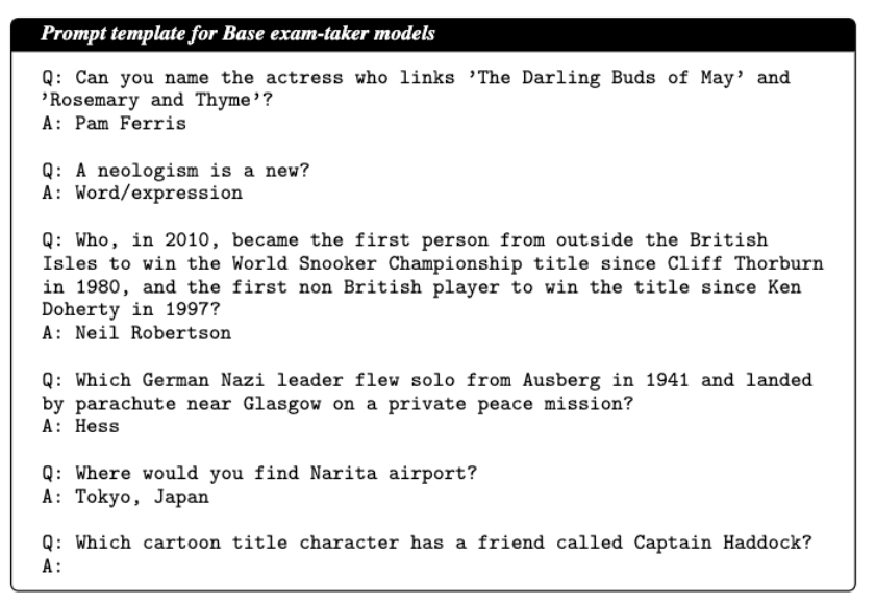
\includegraphics[width=0.8\linewidth]{figures/BaseExamTakerTemplate.pdf}
    \caption{Prompt template for base \evaluatormodels}
    \label{app:template_pretrained}
\end{figure*}

\begin{figure*}[htbp]
    \centering
    \centering
    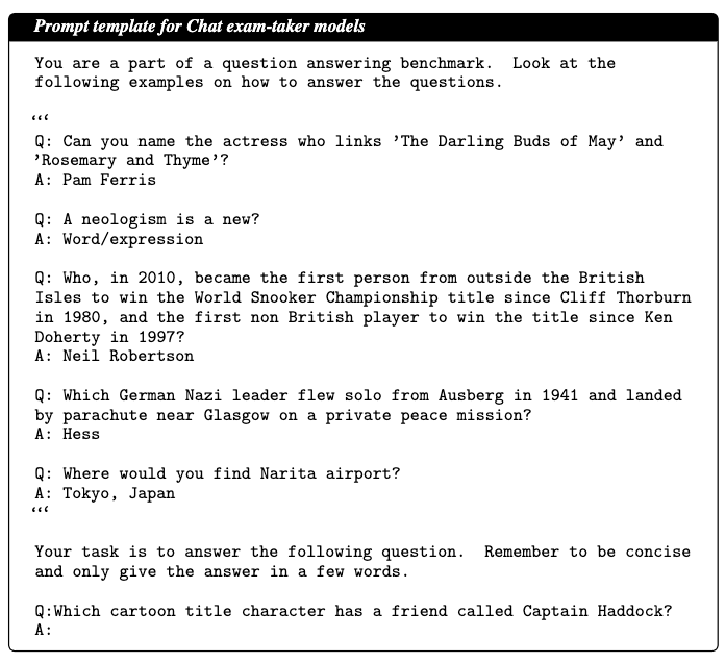
\includegraphics[width=0.8\linewidth, height=0.5\textheight]{figures/ChatExamTakerTemplate.pdf}
    \caption{Prompt template for Chat \evaluatormodels}
    \label{app:template_finetuned}
\end{figure*}


\section{Judge LLM Prompt templates}\label{app:judge-prompt-template}
In \cref{app:WithoutGuidelines}, we show the prompt template used to guide the \judgemodels during the evaluation process of a 400-question sample from the TriviaQA unfiltered dataset.

\begin{figure*}[h]
    \centering
        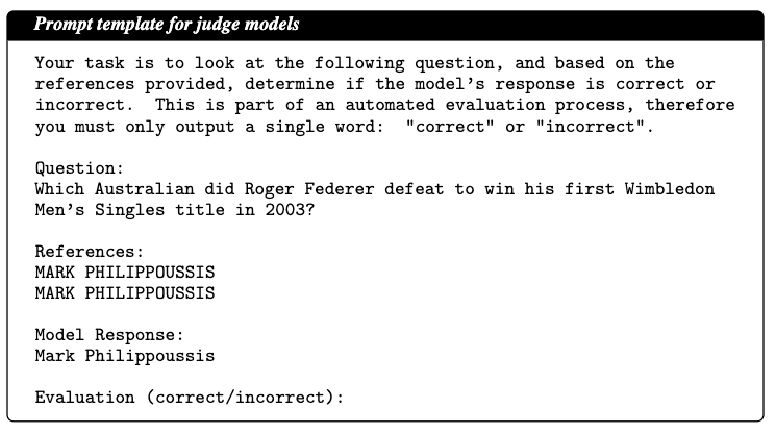
\includegraphics[width=0.8\textwidth, ]{figures/JudgePromptTemplate.pdf}
    \caption{Prompt templates for the \judgemodels}
    \label{app:WithoutGuidelines}
\end{figure*}

\section{Metrics for \judgemodels}
\label{app:metrics}

If one of the annotators is taken to be the reference, then the annotations of the other annotator can be categorized as true positives, false positives, true negatives, and false negatives, with the total number of each of them in a benchmark being represented by $T_P, F_P, T_N,$ and $F_N$ respectively.

\textbf{Percent agreement} is simply the ratio of the numbers of times two annotators agree with each other relative to the total number of annotations. This ratio can have values between $0$ and $1$. For the binary case, the alignment ratio $\rho$ 
%\kc{what symbol to use?} 
is given as

\begin{equation}
    \rho = \frac{T_P + T_N}{T_P + F_P + T_N + F_N}.
\end{equation}

\textbf{Scott's Pi}, \citep{scott1995scottspi}, measures the alignment of two annotators while also taking into account the possibility of agreement by pure chance. This coefficient usually has values above $0$ in most real-world situations. The value of Scott's Pi is given below where $p_o$ is the relative observed agreement, and $p_e$ is the hypothetical probability of chance agreement. 

\begin{figure*}[t]
\begin{equation*}
\pi = \frac{p_o - p_e}{1 - p_e} \nonumber \\
    = \frac{
        \left(\frac{TP + TN}{TP + TN + FP + FN}\right) - 
        \left(\frac{(TP + FP)(TP + FN) + (TN + FN)(TN + FP)}
        {(TP + TN + FP + FN)^2}\right)
    }{
        1 - 
        \left(\frac{(TP + FP)(TP + FN) + (TN + FN)(TN + FP)}
        {(TP + TN + FP + FN)^2}\right)
    }
\end{equation*}
\vspace{-1em}
\label{app:scott-pi}
\end{figure*}

\clearpage
\onecolumn
\section{Human Annotation Guidelines}
\label{app:human_annotation_guidelines}

\mytcolorbox{Human annotation guidelines}{You will be given a question, a set of reference answers and the answer given by an LLM. Your task is to judge if the answer given by the LLM is correct, as if you were the LLMs teacher grading their exam. An answer should be counted as correct if it is semantically equivalent to (one of the) reference answers. In doing so, please follow the following guidelines:}{\begin{itemize}
    \item Underspecified answers (e.g. "December" instead of "December 20") should be marked \textit{incorrect}.
    \item Answers that have more information than requested (e.g. "December 20, in Paris" instead of "December 20") should be marked correct, provided the extra information is not incorrect or contrasting the rest of the answer.
    \item Answers with unnecessary verbosity but correct answers should be marked correct (E.g. ``Thanks for asking this question! The correct answer is: ...").
\end{itemize}
If you have trouble judging whether the answer is correct, for instance because you feel you are lacking knowledge required to judge so, please indicate so by marking the answer "maybe correct" or ``maybe incorrect", so that we can further review it.}

\twocolumn
Preliminary research involved iterative refinement of human annotation guidelines to ensure consistency and reproducibility across annotators with general English semantic knowledge. CS graduate students served as annotators for this experiment. We provide the guidelines used for human evaluation below.

\section{Experiment costs}\label{app:experiment-costs}

The costs for the different experiments described in this work belong in three categories -- GPU-hours for running open-source models on one or more \texttt{Nvidia A100} GPUs, OpenAI credits for making API calls to OpenAI models,\footnote{Pricing details for OpenAI models are available at \url{https://openai.com/api/pricing/}} and human hours for manual annotations of benchmark responses. 
The estimated costs for the final reported experiments are given in \cref{tab:experiment-costs}. 
In addition to this, previous unreported experiments and trials had an approximate cost of 120 GPU-hours, 100 USD in OpenAI credits, and 50 human hours, bringing the total experimental cost for this work to approximately 200 GPU-hours, USD 125 OpenAI credits, and 75 human annotation hours.

\section{Statistical reliability of Evaluation sample} \label{app:downsamplingstddev}

Due to computational constraints discussed in \cref{app:limitations} and \cref{app:experiment-costs}, we limit our evaluation set to randomly sampled 400 questions from TriviaQA \citep{joshi2017triviaqa}. In this section, we further take 5 samples of 300 randomly selected questions from the evaluation set and calculate the mean and standard deviation of Scott's Pi. From \cref{tab:downsampletab}, it can be observed that even on down-sampled sets, the \scottspi values are similar to \cref{fig:llmalignment_b}. Standard deviation of all the \judgemodels from the mean \scottspi is also minimal, barring \judge{EM} lexical match.  

\begin{table}[H]
    \begin{tabular}{lcc}
        \toprule
        Judge Model & Mean \scottspi & Std Dev \\
        \midrule
        Llama3-70B & 0.88 & 0.0046 \\
        Llama3.1-70B & 0.88 & 0.0039 \\
        Llama3.1-8B & 0.78 & 0.0050 \\
        Llama2-13B & 0.75 & 0.0043 \\
        Llama2-70B & 0.69 & 0.0114 \\
        Mistral-7B & 0.67 & 0.0108 \\
        JudgeLM-7B & 0.66 & 0.0026 \\
        Contains & 0.64 & 0.0087 \\
        Llama3-8B & 0.60 & 0.0126 \\
        Llama2-7B & 0.47 & 0.0112 \\
        EM & 0.47  & 0.29 \\
        Gemma-2B & 0.26 & 0.007 \\
        \bottomrule
    \end{tabular}
     \label{tab:downsampletab}
    \centering \captionsetup{skip=8pt} % Adjust space between table and caption
     \caption{Weak \scottspi variation for the 5 down-sampled sets indicating robustness for the evaluation sample}
\end{table}

\section{Judge Scores}
\label{app:all_scores}

We show the scores assigned by each \judgemodel to each \evaluatormodel, visualised in \cref{fig:llmalignment_a} in \cref{tab:eval-scores}.



% \section{Too Much Info Confuses the LLM}
% \label{app:TMI}
% \textcolor{red}{v1 and v2}
% Here are the prompt templates used for this experiment. The simplest prompt used is \textit{Without Guidelines v1} (see \cref{app:WithoutGuidelines_v1}) where we define a sequential and structured process for the \judgemodel. In \textit{Without Guidelines v2} (see \cref{app:WithoutGuidelines_v2}), we add an additional focus on the overall task and outcome as well. 

% For \textit{Guidelines without examples} (see \cref{app:GuidelinesWithoutExamples}), we provide the \judgemodels with detailed instructions about the task at hand, along with explicit guidelines on how to evaluate the answers. Additionally, for \textit{Guidelines with examples}(see \cref{app:GuidelinesWithExamples}), we also provide examples to the \judgemodels for further reference.

\section{\Evaluatormodel base vs chat analysis}
\label{app:BaseVsChatSupp}

Given the human judgments we have available, we take the opportunity to investigate the performance differences between base and their corresponding chat models.
In \cref{tab:ScoresBaseChat}, we show the scores assigned by various \judgemodels to four base-chat pairs.
According to the default metric \judge{EM}, the base models outperform the chat models by a large margin.
Interestingly, while this difference gets smaller when the answers are judged by humans (second column) or \judge{GPT-4 Turbo}, there is still a substantial difference for all four pairs, suggesting that the difference is not merely an effect of the increased verbosity of the chat models.
Further evidence for that hypothesis is provided by \cref{fig:BaseChatPieChart}, in which we can see that while 14\% of the errors are shared between the base-chat pairs, almost another 14\% of the examples get judged correctly by the base models but not by the chat models, while the opposite happens in only 2.5\% of the cases.

\onecolumn
\begin{table}[H]
    \centering
    \begin{tabular}{lccc}
        \toprule
        Experiment & GPU-hours & OpenAI credits & Human hours \\
        \midrule
        Main benchmarks & 5 & 2 & - \\
        Main evaluations & 30 & 8 & 10 \\
        Human alignment & 2 & - & 9 \\
        Error analysis & 1.5 & - & 5 \\
        Controlled responses & 15 & - & - \\
        Leniency bias & 5 & 5 & - \\
        Guideline bias & 10 & 5 & 1 \\
        Reference bias & 5 & 4 & 1 \\
        \midrule
        \textbf{Total} & \textbf{73.5} & \textbf{24} & \textbf{26} \\
        \bottomrule
    \end{tabular}
    \label{tab:experiment-costs}
         \captionsetup{skip=8pt} % Adjust space between table and caption
     \caption{Estimated costs for the final reported experiments. GPU-hours are in equivalent \texttt{Nvidia A100} hours, OpenAI credits are in USD, and human hours are time spent in manual annotation.}
\end{table}

\begin{table}[h]
\label{tab:eval-scores}
\centering
    % \begin{tabular}{cccc@{\extracolsep{2mm}}ccc@{\extracolsep{2mm}}ccc@{\extracolsep{2mm}}c}
    \setlength{\tabcolsep}{5pt}
    \begin{tabular}{ccccccccccc}
    % \toprule
% \small
    &  \multicolumn{9}{c}{\textbf{Exam taker models}} \\
    \cmidrule{2-10}
    & \multicolumn{6}{c}{Llama2} & \multicolumn{2}{c}{Mistral} & GPT-4 \\ 
    & \multicolumn{3}{c}{Base} & \multicolumn{3}{c}{Chat} & Base & Instruct \\
% \begin{longtable}{|p{1.4cm}|p{1.1cm}|p{1.1cm}|p{1.1cm}|p{1.1cm}|p{1.1cm}|p{1.1cm}|p{1.1cm}|p{1.1cm}|p{1.1cm}|p{1.1cm}|}
% \hline
% \multicolumn{2}{|c|}{\multirow{2}{*}{}} & \multicolumn{9}{|c|}{\textbf{Exam Taker Models}} \\ \cline{3-11}
% \multicolumn{2}{|c|}{\multirow{2}{*}{}} & \multicolumn{6}{c|}{Llama 2} & \multicolumn{2}{c|}{Mistral} & \multicolumn{1}{c|}{} \\ \cline{3-11}
% \multicolumn{2}{|c|}{} & \multicolumn{3}{c|}{Base} & \multicolumn{3}{c|}{Chat} & \multicolumn{1}{c|}{Base} & \multicolumn{1}{c|}{Instruct} &  \\ \hline
\textbf{Judge Models} & 7B  & 13B & 70B & 7B & 13B & 70B & \multicolumn{2}{c}{7B} \\
\cmidrule[1pt]{2-10}
Llama 3.1 8B & 65.25 & 75.00 & 83.50 & 60.25 & 70.50 & 75.50 & 73.75 & 59.00 & \textbf{89.00} \\ 
Llama 3.1 70B & 62.00 & 74.25 & 85.00 & 55.50 & 64.75 & 74.00 & 72.25 & 60.50 & \textbf{92.25} \\ \midrule
Llama 3 8B & 76.00 & 83.25 & 91.50 & 73.25 & 82.75 & 85.25 & 81.75 & 76.0 & \textbf{97.25} \\ 
Llama 3 70B & 64.25 & 75.50 & 86.50 & 57.00 & 64.00 & 75.75 & 73.5 & 62.50 & \textbf{92.75} \\ \midrule
Llama 2 7B & 80.50 & 85.25 & 92.00 & 80.50 & 70.75 & 90.75 & 84.00 & 83.25 & \textbf{97.75} \\ 
Llama 2 13B & 68.25 & 75.50 & 86.50 & 63.25 & 62.75 & 77.50 & 74.50 & 67.50 & \textbf{93.5} \\ 
Llama 2 70B & 71.25 & 80.5 & 90.25 & 67.50 & 74.75 & 81.25 & 80.0 & 72.5 & \textbf{96.75} \\ \midrule
Mistral 7B & 72.50 & 80.75 & 90.50 & 69.00 & 74.75 & 82.50 & 80.25 & 72.00 & \textbf{96.25} \\ \midrule
Gemma 2B & 79.75 & 87.00 & \textbf{91.25} & 58.50 & 41 & 68.50 & 84.0 & 55.75 & 80.50 \\ \midrule
JudgeLM & 69.50 & 77.75 & 86.25 & 63.75 & 48.0 & 82.75 & 77.25 & 71.0 & \textbf{94.50} \\ \midrule
GPT-4 & 60.50 & 71.50 & 82.50 & 54.50 & 59.0 & 73.0 & 69.75 & 56.50 & \textbf{90.0} \\ \midrule
Exact Match & 46.75 & 56.00 & \textbf{63.75} & 24.00 & 0.25 & 36.25 & 59.50 & 20.25 & 58.25 \\ 
Contains Match & 50.75 & 60.00 & 68.00 & 39.00 & 46.25 & 59.50 & 57.25 & 44.00 & \textbf{70.00} \\ \midrule
Human Eval & 62.50 & 72.75 & 83.75 & 56.00 & 56.50 & 72.25 & 71.75 & 60.75 & \textbf{91.50} \\
\bottomrule
\end{tabular}
 \captionsetup{skip=8pt} % Adjust space between table and caption
\caption{\Judgemodel score card for every \evaluatormodel.}
\end{table}

\twocolumn




% \begin{subfigure}[b]{0.6\textwidth}
% \renewcommand{\arraystretch}{0.7} % Reduce row spacing
% \setlength{\tabcolsep}{3pt} % Reduce column spacing
% \begin{tabular}{@{}lrrrrr@{}}
% \toprule
% \multicolumn{1}{c}{} & \multicolumn{5}{c}{\textbf{Judge models}} \\ \cmidrule(lr){2-6}
% \makecell{Base-Chat\\ pair} & EM & Human & \makecell{GPT-4\\Turbo} & \makecell{Llama-2\\70B} & \makecell{Llama-2\\7B} \\ \midrule
% \makecell{Llama-2\\7B} & 22.75 & 6.25 & 6.50 & 4.25 & 3.25 \\ \cmidrule(lr){1-6}
% \makecell{Mistral\\7B} & 39.25 & 11.00 & 19.75 & 2.75 & -11.75 \\ \cmidrule(lr){1-6}
% \makecell{Llama-2\\13B} & 55.25 & 16.25 & 17.50 & -3.75 & -6.00 \\ \cmidrule(lr){1-6}
% \makecell{Llama-2\\70B} & 27.50 & 11.50 & 13.00 & 4.25 & 22.25 \\ \bottomrule
% \end{tabular}
% \caption{}
% \label{tab:DeltaValuesBaseChat}
% \end{subfigure}

\begin{table}[b]
    \centering
\label{tab:ScoresBaseChat}
 \captionsetup{skip=8pt} % Adjust space between table and caption
\caption{Scores of base and chat models by various judges}
\setlength{\tabcolsep}{6pt}
\begin{tabular}{p{2.5cm}cccccccccc}
\toprule
& \multicolumn{10}{c}{\textbf{Judge models}} \\ \cmidrule(lr){2-11}
    \makecell{Base-Chat\\ pair} & \multicolumn{2}{c}{EM} & \multicolumn{2}{c}{Contains} & \multicolumn{2}{c}{Human} & \multicolumn{2}{c}{\makecell{GPT-4\\Turbo}} & \multicolumn{2}{c}{\makecell{Llama-3\\70B}} \\
    \cmidrule{2-11}
    & Base & Chat & Base & Chat & Base & Chat & Base & Chat & Base & Chat \\
    \makecell{Llama-2 7B} & \textbf{46.75} & 24.00 & \textbf{50.75} & 39.00 & \textbf{62.25} & 56.00 & \textbf{60.50} & 54.50 & \textbf{64.25} & 57.00\\
    \makecell{Mistral 7B} & \textbf{59.50} & 20.25 & \textbf{57.25} & 44.00 & \textbf{71.75} & 60.75 & \textbf{69.75} & 56.50 & \textbf{73.50} & 62.50\\
    \makecell{Llama-2 13B} & \textbf{ 56.00} & 0.25 & \textbf{60.00} & 46.25 & \textbf{72.75} & 56.50 & \textbf{75.00} & 59.00 & \textbf{76.50} & 64.00\\
    \makecell{Llama-2 70B} & \textbf{63.75} & 36.25 &  \textbf{68.00} & 59.50 & \textbf{83.75} & 72.25 & \textbf{82.50} & 73.00 & \textbf{86.50} & 75.75\\
\bottomrule
\end{tabular}
\end{table}

We consider two alternative hypotheses:\begin{itemize}\setlength\itemsep{0.1em}
    \item[i)] The chat models have a worse understanding of the particular prompt format, which is tuned more to fit base models; or
    \item[ii)] The chat models have `unlearned' some knowledge during their alignment training.
\end{itemize}

To disentangle these two factors, we manually analyse 400 questions for \eval{Llama-2 70B} and \eval{Llama-2 70B-chat}, using our earlier error codes.
The results, shown in \cref{fig:comparisonBarplot}, sugest that, at least to some extent, the difference between base and chat models is in fact due to `unlearning' of knowledge: while the number of errors is more or less equal among most categories, there is a stark difference in the \emph{incorrect entity} category.
Substantially more often than the base models, the chat models do answer the question with a semantically plausible but incorrect entity.
In \cref{tab:KnowledgeUnlearningExample1}-\cref{tab:KnowledgeUnlearningExample3}, we provide examples of such cases.
The results do not show any evidence to support the first hypothesis: the number of errors where the answer cannot be parsed or is just entirely incorrect does not differ between base and chat models.

\section{\Evaluatormodel ranking correlation }
\label{app:correlationcoefftable}
% In \cref{tab:judges_rho_reversed}, we show the Spearman's rank correlation coefficient \citep{spearman1904spearman} ($\rho$) with human judgment. 
% Since $\rho$ > 0.7 is considered well aligned, only \judge{Llama-7B and \judge{Gemma-2B} have poor rank correlation with human judgment.} 


In \cref{tab:judges_rho_reversed}, We use the Spearman Rank correlation coefficient  \citep{spearman1904spearman} to assess the rankings of the \evaluatormodels. To validate these rankings, we randomly select 6 out of \nexamtakers \evaluatormodels across 5 samples, subsequently calculating the mean ($\rho$) and standard deviation ($\sigma$) of the rankings. The results reveal that the \judge{contains} model exhibits the highest stability and $\rho$ among the rankings, while the majority of judge models achieve a coefficient exceeding 0.7, indicating a strong alignment. Notably, smaller models such as \judge{Mistral 7B} perform on par with \judge{\gpt}, highlighting the robustness of smaller models in maintaining rankings.

\begin{table}[H]
\label{tab:judges_rho_reversed}
    \centering
    \begin{tabular}{lcc}
        \toprule
        Judges & $\rho$ & $\sigma$ \\
        \midrule
        Contains & 0.99 & 0.02 \\
        Mistral-7B & 0.98 & 0.03 \\
        GPT-4 & 0.98 & 0.03 \\
        Llama2-13B & 0.95 & 0.18 \\
        JudgeLM-7B & 0.95 & 0.05 \\
        Llama2-7B & 0.94 & 0.04 \\
        Llama3.1-70B & 0.94 & 0.07 \\
        Llama3-70B & 0.93 & 0.05 \\
        Llama3.1-8B & 0.89 & 0.10 \\
        Llama3-8B & 0.86 & 0.07 \\
        Llama2-70B & 0.84 & 0.13 \\
        Gemma-2B & 0.71 & 0.20 \\
        EM & 0.67 & 0.13 \\
        \bottomrule
    \end{tabular}
            \captionsetup{skip=5pt}
    \caption{Spearman Rank Correlation Coefficient $\rho$.}
\end{table}

% \clearpage
\section{Too much info confuses judges}
\label{app:TMI}
In \cref{app:WithoutGuidelines_v1}-\ref{app:GuidelinesWithExamples}, we report the guidelines we used for the experiments in \cref{sec:analysis:subsec:instructions}. 
The simplest prompt used is \textit{Without Guidelines v1} (see \cref{app:WithoutGuidelines_v1}) where we define a sequential and structured process for the \judgemodel. 
In \textit{Without Guidelines v2} (see \cref{app:WithoutGuidelines_v2}), we add an additional focus on the overall task and outcome as well. 
% 
For \textit{Guidelines without examples} (see \cref{app:GuidelinesWithoutExamples}), we provide the \judgemodels with detailed instructions about the task at hand, along with explicit guidelines on how to evaluate the answers. 
Additionally, for \textit{Guidelines with examples}(see \cref{app:GuidelinesWithExamples}), we also provide examples to the \judgemodels for further reference.


% \begin{itemize}[noitemsep]
% \item Knowledge unlearning by the chat models or Loss in knowledge (Correct Answer by Base model and Wrong Answer by Chat model) - $\mathcal{L}_{knowledge}$
% \item Error in judgment by \judgemodels (Right answer by Chat model but wrong judgment or Wrong answer by Base model but judged as right) - $\epsilon$
% \item Misc (Chat model fails to understand the prompt or answer Cut off) - $\mu$
% \end{itemize}

% \[
% \begin{array}{cc}
% \Delta_{\text{Human}} = \mathcal{L}_{knowledge} + \mu & \hspace{2cm} \Delta_{\text{LLM}} = \mathcal{L}_{knowledge} + \mu \pm \epsilon
% \end{array}
% \]

%%%%%%%%%%%%%%%%%%%%%%%%%
% Storyline
% 1) First we show the difference in scores and show not many 'Answer cut off' or other errors for chat models and hence its mostly Knowledge unlearning that contributes to delta in scores between Base and Chat models
% 2) Then we have to explain why is the delta varying across all judge models since Knowledge unlearning is same no matter what judge model we use. So here we say that its upto the judge model. Bigger judge = lineant scoring, smaller judge = harsher. Hence decrease in delta. Additionally, Knowledge unlearning is greater in bigger Base-Chat pairs
%%%%%%%%%%%%%%%%%%%%%%%%%%

% Assuming there is zero error in human judgment, $\epsilon$ in $\Delta_{\text{Human}}$ = 0. 

% The plots in \cref{fig:BaseChatPieChart} and \cref{fig:comparisonBarplot} suggest knowledge unlearning, as the Chat model provides more incorrect answers than the Base model, with the majority of these errors classified as 'incorrect entities' or 'under specification' (examples in \cref{app:BaseVsChatSupp}). 
% Specifically, \cref{fig:comparisonBarplot} shows that the \eval{Llama2 70B} Chat model answers a higher number of questions as 'incorrect entity' compared to the corresponding base model. 
% Furthermore, the Chat model provides too few entities in more responses than the Base model, indicating knowledge unlearning due to its inability to provide all the required entities for correct answers.
\onecolumn
\begin{figure}[t]
\centering
\begin{subfigure}{0.6\textwidth}
    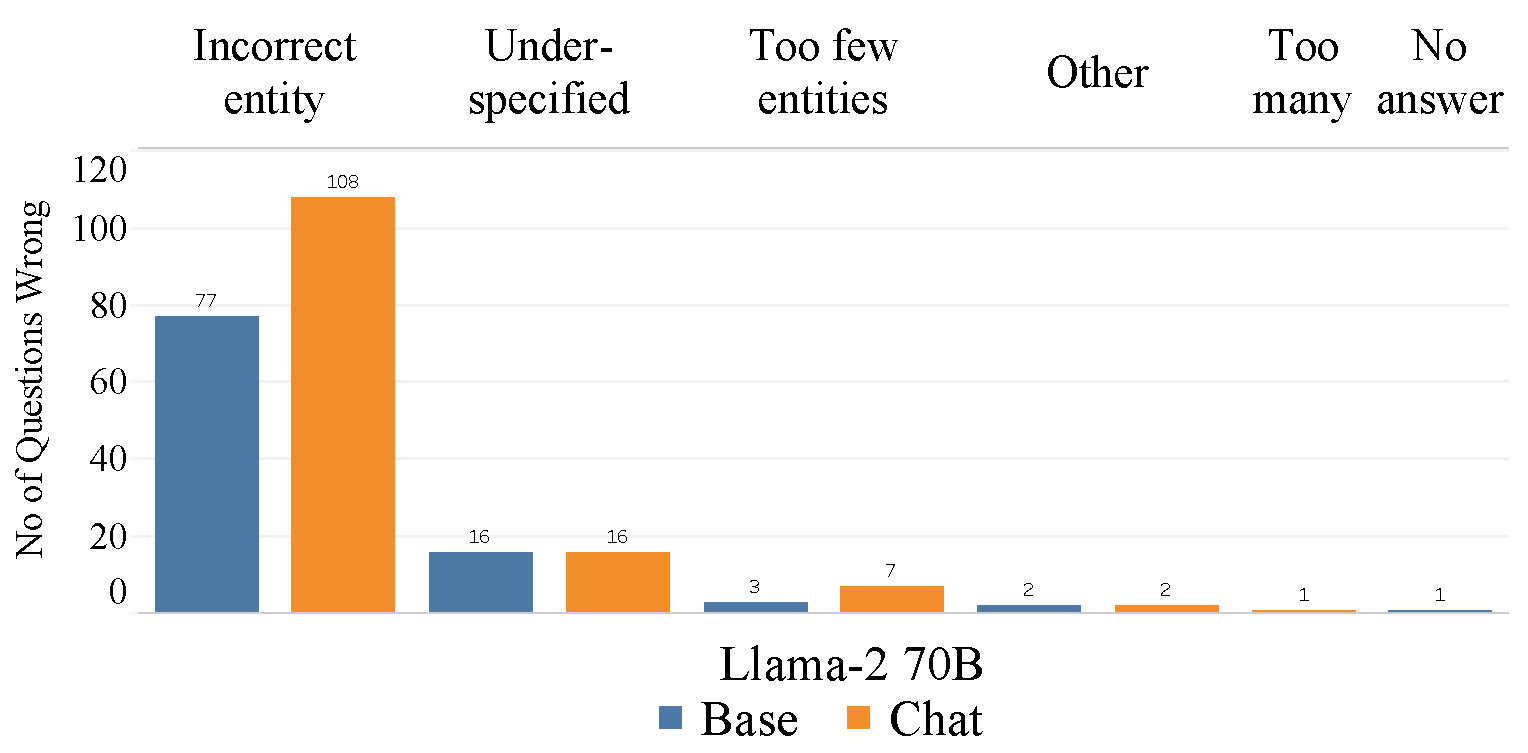
\includegraphics[width=\textwidth]{figures/ErrorCode.pdf}
    \caption{}
     \label{fig:comparisonBarplot}
\end{subfigure}
%
\hfill
%
\begin{subfigure}{0.39\textwidth}
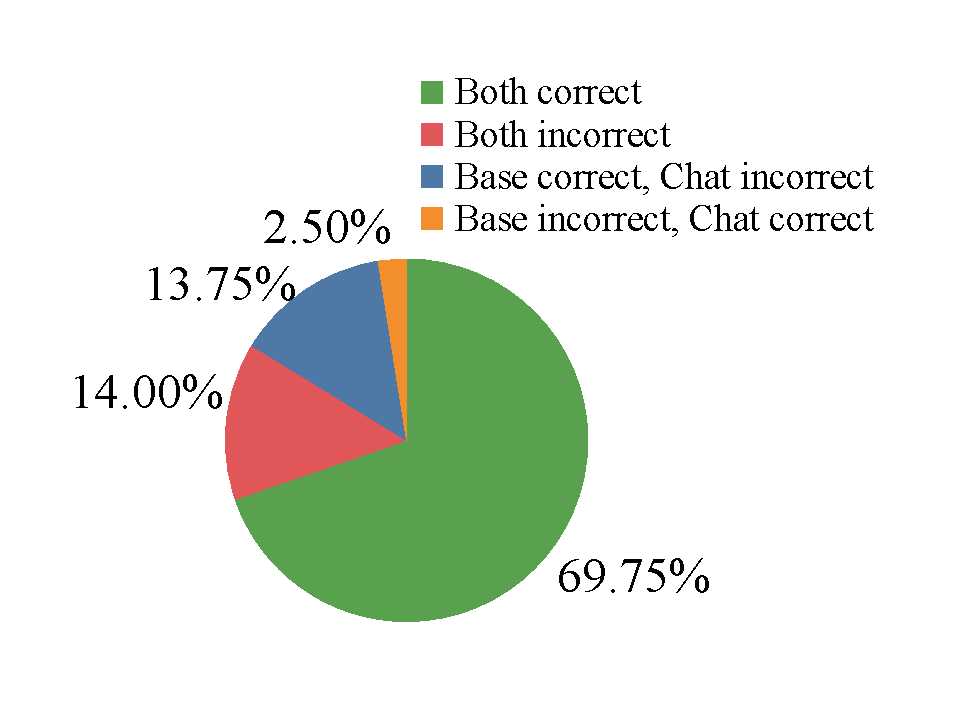
\includegraphics[width=\textwidth]{figures/PieChart.pdf}
% \vspace{15pt}
\caption{}
\label{fig:BaseChatPieChart}
\end{subfigure}
\caption{a) Distribution of incorrect question counts by error codes for \eval{Llama2 70B} Base vs Chat \evaluatormodels evaluated on 400 questions. b) Pie chart showing the percentage of questions categorized by the judgment from Base and Chat models.}
\end{figure}



% Additionally, \cref{fig:BasevsChat} shows with an increase in model size, \judge{GPT-4 Turbo} as a judge has a similar Kappa and alignment score with humans only for the Chat models. This implies that while bigger \judgemodels effectively parse and evaluate the verbose responses from the chat models, the main problem lies in the accuracy of their answers, which leads to a lower judge score and further suggesting knowledge unlearning.

% Furthermore, \cref{fig:BasevsChat} demonstrates that although the Llama-2 Base models have higher judge scores compared to the Chat models, the $\kappa$ score and percent agreement of \judge{GPT} increase for the Chat models and decrease for the Base models as the model size grows. 
% This indicates that the issue with the Chat models lies in the accuracy of their answers, resulting in lower judge scores, rather than an error in parsing their verbose responses. 
% This further suggests the unlearning of knowledge by the Chat models.

% Interestingly, across all \judgemodels, as the size of the \evaluatormodel increases, $\Delta$ also increases, suggesting that $\mathcal{L}_{knowledge}$ between the Base and Chat models widens as the model size grows. % \dieuwke{This doesn't seem to be true to me from the numbers: Llama 2 70B has a smaller difference than Llama-2 13B.

%Moreover, as the \judgemodel size gets smaller, the $\Delta_{\text{LLM}}$ values decreases, well beyond the observed $\Delta_{\text{Human}}$. 
% Given that $\mathcal{L}_{knowledge}$ and $\mu$ remain constant across all the \judgemodels, the only variable changing here is $\pm \epsilon$. 

% The scores from \cref{tab:eval-scores} indicate that the base \evaluatormodels are evaluated more strictly, while the chat \evaluatormodels are evaluated too leniently by the smaller \judgemodels. 
% This results in $\Delta_{\text{LLM}}$s that are smaller and sometimes negative, in contrast to the absolute scores that deviate significantly from the true scores. 
% One possible explanation is that the smaller \judgemodels are tricked by the verbose responses of the Chat \evaluatormodels into rewarding them with higher scores. However, this does not hold true for the larger \judgemodels.

% \begin{figure}[H]
% \centering
%     \centering
%     \includegraphics[width=\textwidth]{figures/BasevsChat.pdf}
%     \caption{Evaluation Metrics for LLama2 Base and Chat \evaluatormodel pairs evaluated by \judge{GPT-4 Turbo}}
%     \label{fig:BasevsChat}
% \end{figure}
\definecolor{darkgreen}{rgb}{0.0, 0.5, 0.0}
\begin{table}[H]
\centering
\label{tab:KnowledgeUnlearningExample1}
\begin{tabular}{|>{\raggedright\arraybackslash}m{2.5cm}|>{\raggedright\arraybackslash}m{10cm}|}
\hline
\multicolumn{2}{|c|}{\textbf{Question:}} \\
\multicolumn{2}{|c|}{\texttt{Which British artist's works include `The First Real Target'?}} \\
\hline
\textbf{References} & \rule{0pt}{3ex}\texttt{Peter Blake, Peter Balke, Sir Peter Blake}\rule[-1ex]{0pt}{1ex} \\
\hline
\textbf{LLama-2 70B Base} & \rule{0pt}{3ex}\textcolor{darkgreen}{\texttt{Peter Blake}}\rule[-1ex]{0pt}{1ex} \\
\hline
\textbf{LLama-2 70B Chat} & \rule{0pt}{3ex}\textcolor{red}{\texttt{Patrick Caulfield}}\rule[-1ex]{0pt}{1ex} \\
\hline
\textbf{Mistral 7B Base} & \rule{0pt}{3ex}\textcolor{red}{\texttt{David Hockney}}\rule[-1ex]{0pt}{1ex} \\
\hline
\textbf{Mistral 7B Chat} & \rule{0pt}{3ex}\textcolor{red}{\texttt{Damien Hirst}}\rule[-1ex]{0pt}{1ex} \\
\hline
\end{tabular}
\label{tab:KnowledgeUnlearningExample1}
\captionsetup{skip=5pt}
\caption{Knowledge unlearning example 1.}
\end{table}

\begin{table}[H]
\label{tab:KnowledgeUnlearningExample2}
\centering
\begin{tabular}{|>{\raggedright\arraybackslash}m{2.5cm}|>{\raggedright\arraybackslash}m{10cm}|}
\hline
\multicolumn{2}{|c|}{\textbf{Question:}} \\
\multicolumn{2}{|c|}{\texttt{Who was the first cricketer to score 10,000 test runs?}} \\
\hline
\textbf{References} & \rule{0pt}{3ex}\texttt{Sunil Gavaskar, Sunil Manohar Gavaskar, SM Gavaskar, Sunny gavaskar, Gavaskar}\rule[-1ex]{0pt}{1ex} \\
\hline
\textbf{LLama-2 70B Base} & \rule{0pt}{3ex}\textcolor{darkgreen}{\texttt{Sunil Gavaskar}}\rule[-1ex]{0pt}{1ex} \\
\hline
\textbf{LLama-2 70B Chat} & \rule{0pt}{3ex}\textcolor{red}{\texttt{Sachin Tendulkar}}\rule[-1ex]{0pt}{1ex} \\
\hline
\textbf{Mistral 7B Base} & \rule{0pt}{3ex}\textcolor{red}{\texttt{Sachin Tendulkar}}\rule[-1ex]{0pt}{1ex} \\
\hline
\textbf{Mistral 7B Chat} & \rule{0pt}{3ex}\textcolor{red}{\texttt{Sachin Tendulkar}} \texttt{was the first cricketer to score 10,000 runs in Test matches.}\rule[-1ex]{0pt}{1ex} \\
\hline
\end{tabular}
\label{tab:KnowledgeUnlearningExample2}
\captionsetup{skip=5pt}
\caption{Knowledge unlearning example 2}
\end{table}


\begin{table}[H]
\label{tab:KnowledgeUnlearningExample3}
\centering
\begin{tabular}{|>{\raggedright\arraybackslash}p{2.5cm}|>{\raggedright\arraybackslash}p{10cm}|}
\hline
\multicolumn{2}{|c|}{\textbf{Question:}} \\
\multicolumn{2}{|c|}{\parbox{12cm}{\texttt{`Uncle Harry's Coat' was the first garment produced by which famous jacket manufacturer, based in Simonside, Newcastle Upon Tyne?}}} \\
\hline
\textbf{References} & \rule{0pt}{3ex}\texttt{Barbour}\rule[-1ex]{0pt}{1ex} \\
\hline
\textbf{LLama-2 70B Base} & \rule{0pt}{3ex}\textcolor{darkgreen}{\texttt{Barbour}}\rule[-1ex]{0pt}{1ex} \\
\hline
\textbf{LLama-2 70B Chat} & \rule{0pt}{3ex}\textcolor{darkgreen}{\texttt{Barbour}}\rule[-1ex]{0pt}{1ex} \\
\hline
\textbf{Mistral 7B Base} & \rule{0pt}{3ex}\textcolor{darkgreen}{\texttt{Barbour}}\rule[-1ex]{0pt}{1ex} \\
\hline
\textbf{Mistral 7B Chat} & \rule{0pt}{3ex}\textcolor{red}{\texttt{Jack Walker \& Sons}}\rule[-1ex]{0pt}{1ex} \\
\hline
\end{tabular}
\label{tab:KnowledgeUnlearningExample3}
\captionsetup{skip=5pt}
\caption{Knowledge unlearning example 3}
\end{table}

\clearpage

\begin{figure}[H]
    \centering
    \resizebox{0.8\textwidth}{!}{
        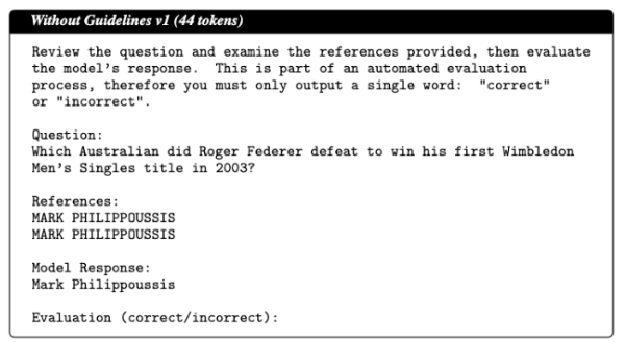
\includegraphics{figures/WithoutGuidelinesv1.pdf}
    }
    \caption{\textit{Without Guidelines v1} prompt template for the \judgemodels}
    \label{app:WithoutGuidelines_v1}
\end{figure}

\begin{figure}[t]
    \centering
    \resizebox{0.8\textwidth}{!}{
        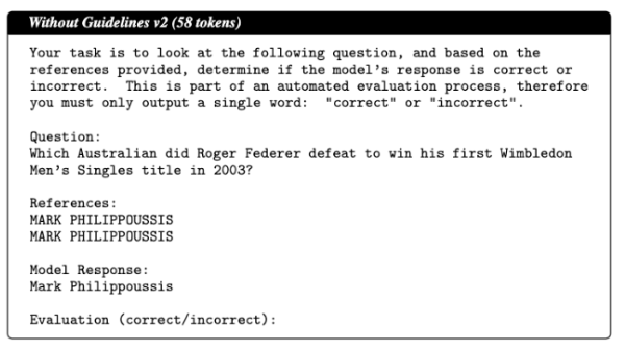
\includegraphics{figures/WithoutGuidelinesv2.pdf}
    }
    \caption{\textit{Without Guidelines v2} prompt template for the \judgemodels}
    \label{app:WithoutGuidelines_v2}
\end{figure}

\begin{figure}[h]
    \centering
    \resizebox{0.7\textwidth}{!}{
        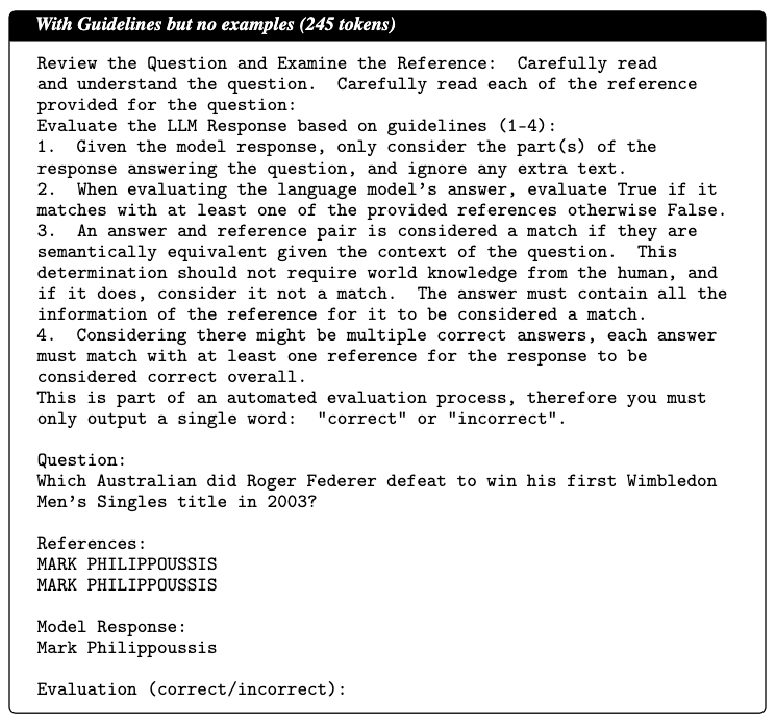
\includegraphics{figures/WithGuidelinesNoExamples.pdf}
    }
    \caption{\textit{Guidelines without examples} Prompt template for the \judgemodels}
    \label{app:GuidelinesWithoutExamples}
\end{figure}

% \vspace{-0.75cm}

\begin{figure}[ht]
    \centering
    \resizebox{0.7\textwidth}{!}{
        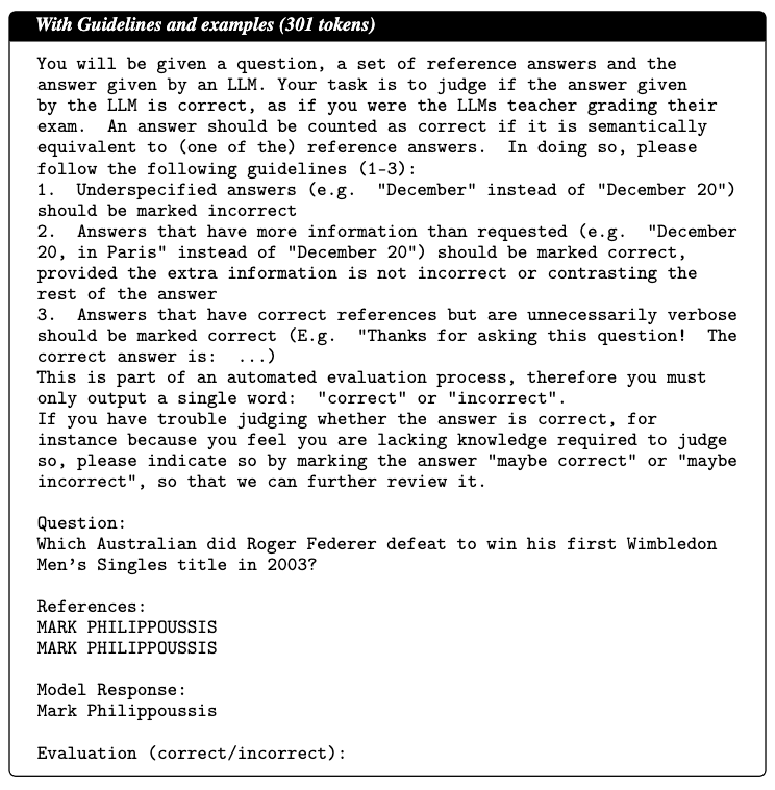
\includegraphics{figures/WithGuidelinesAndExamples.pdf}
    }
    \caption{\textit{Guidelines with Examples} Prompt template for the \judgemodels}
    \label{app:GuidelinesWithExamples}
\end{figure}

% \begin{table}[h]
%     \centering
%     \small
%     \setlength{\tabcolsep}{4pt} % Adjust column separation
%     \renewcommand{\arraystretch}{1.2} % Adjust row separation
%     \begin{tabular}{p{2.5cm}|p{1.0cm}|p{1.0cm}|p{1.0cm}|p{1.0cm}|p{1.0cm}}
%     \toprule
%     \makecell[l]{Prompt\\Template} & \makecell[l]{Llama-2\\7B} & \makecell[l]{Llama-2\\13B} & \makecell[l]{Llama-2\\70B} & \makecell[l]{Mistral\\7B} & \makecell[l]{GPT-4} \\
%     \midrule
%     \makecell[l]{Without \\ Guidelines v1 (44)} & 0.66 & 0.67 & \textbf{0.87} & 0.68 & 0.87 \\
%     \midrule
%     \makecell[l]{Without \\ Guidelines v2 (58)} & \textbf{0.67} & \textbf{0.73} & 0.82 & \textbf{0.75} & 0.89 \\
%     \midrule
%     \makecell[l]{Guidelines \\ w/o Examples (245)} & 0.43 & 0.42 & 0.73 & \textbf{0.75} & \textbf{0.93} \\
%     \midrule
%     \makecell[l]{Guidelines \\ with Examples (301)} & 0.39 & \textbf{0.73} & 0.70 & 0.61 & 0.90 \\
%     \bottomrule
%     \end{tabular}
%     \vspace{6pt} % Adjust the space here
%     \caption{Kappa scores with humans for various \judgemodels across different prompt templates.}
%     \label{tab:TMI_Kappa}
% \end{table}

\begin{figure}[htbp]
    \centering
    \resizebox{0.6\textwidth}{!}{
        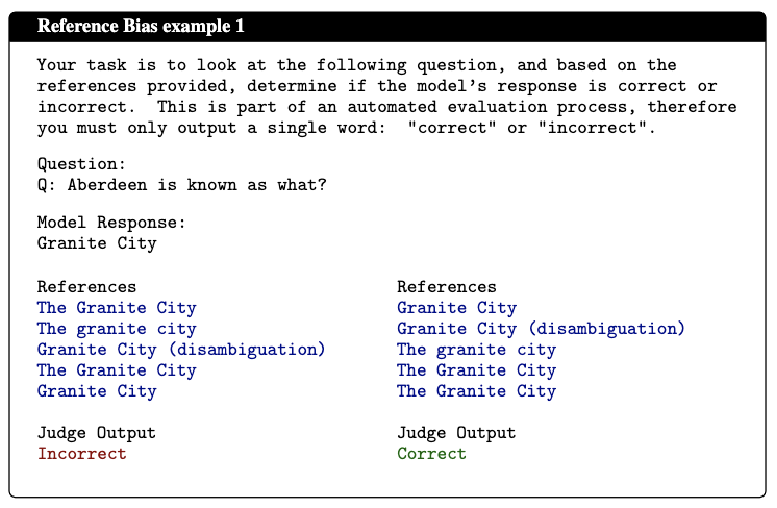
\includegraphics{figures/ReferenceBiasExample1.pdf}
    }
    \caption{Example of \judge{Llama2-7B} getting confused when the order of the references are changed}
    \label{app:ReferenceBiasExample1}
\end{figure}

\begin{figure}[H]
    \centering
    \resizebox{0.6\textwidth}{!}{
        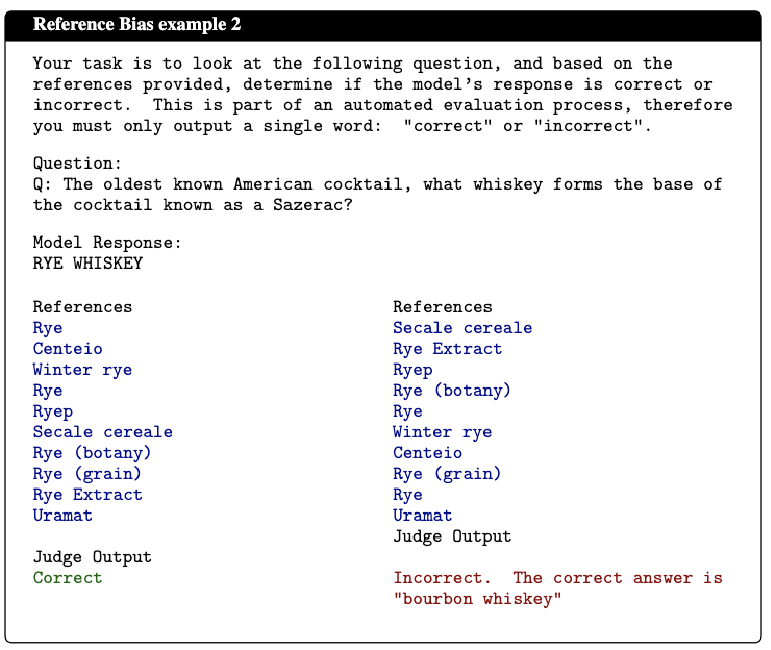
\includegraphics{figures/ReferenceBiasExample2.pdf}
    }
    \caption{Example of \judge{Llama2-7B} failing to identify the task by changing the order of the references.}
    \label{app:RefernceBiasExample2}
\end{figure}

\clearpage
\twocolumn
\section{\Judgemodels are sensitive to reference order}
\label{app:ref-bias-exp}

We investigate the judges' sensitivity to reference order by providing the same prompt, question and model response to the \judgemodels, but shuffling the reference order in three different permutations. We compute the consistency score of the model as the percentage of questions for which it gives the same judgment all the 3 times. 
%
% \dieuwke{Give formula of how we compute it.}
We observe that the model is more likely to evaluate an answer as correct if the corresponding reference appears early in the list of references (see \cref{app:ReferenceBiasExample1}).
% Additionally another factor that makes a judge LLM a good judge is consistency.
%
The smaller \judgemodels sometimes fail to capture all the information in the prompt, and provide judgement based on their own knowledge rather than going by the references (see  \cref{app:RefernceBiasExample2}).

% \begin{figure}[H]
%     \centering
%     \resizebox{0.9\textwidth}{!}{
%         \includegraphics{figures/Consistency_Plot.pdf}
%     }
%     \caption{Consistency Score and Average Kappa score with Humans for different \judgemodels for 3 random reference order permutation runs}
%     \label{app:GuidelinesWithExamples}
% \end{figure}
% \begin{table}[H]
% \centering
% \vspace{0.5em} % Adjust the spacing here
% \begin{tabular}{|c|c|c|c|c|c|c|c|c|}
% \hline
% & Exact-match & Llama2 7B & Llama2 13B & Llama2 70B & Mistral 7B & GPT 4T \\
% \hline
% Default & 42.00 & 49.50 & 52.50 & 62.00 & 61.50 & 57.25\\
% \hline
% Shuffled & 42.00 & 48.50 & 54.25 & 61.75 & 61.75 & 57.75\\
% \hline
% \end{tabular}
% \vspace{1em} % Adjust the spacing between caption and table
% \caption{judgment Scores for different ordering of the references given during judging for Llama-7B Base as the Exam-taker model}\label{table:reference_consistency}
% \end{table}


\section{Leniency Bias}\label{app:leniency-bias}

As described in \cref{sec:leniency-bias}, for the purpose of the leniency bias experiments, we assume that a judge assigns the correct judgment with a probability of $P_c$ and randomly assigns the rest of the samples to be \texttt{“correct”} with a probability $P_+$.
%
In this section, we derive the mathematical expressions for $P_c$ and $P_+$. We assume that in the case of misalignment between the evaluation criteria of guidelines and \judgemodels, the probability of getting an evaluation of \texttt{``correct''} is independent of the actual correctness of the answer (i.e.\ the \judgemodel effectively flips a coin to give out its judgement). For any given benchmark and \judgemodel, we denote the ground-truth score as $s$, and the true positive and true negative rates as $t_P$ and $t_N$, respectively, all normalized to be between $0$ and $1$.

Now, based on our assumptions, the true positives, where the \evaluatormodel response is correct, and also correctly identified by the \judgemodel to be correct, would be comprised of two possible cases: 1) The judge evaluates it correctly according to the given evaluation criteria with a probability of $P_c$; and 2) The judge does not evaluate it according to the given criteria with a probability of $1-P_c$, but the evaluation still happens to be correct with a probability of $P_+$. With the total ratio of the correct responses being $s$, the true positive rate is therefore given by --

\begin{equation}\label{eq:tp}
    t_P = s[P_c + (1-P_c)P_+]
\end{equation}

Similarly, the true negatives, where the \evaluatormodel response is incorrect, and also correctly identified by the \judgemodel to be incorrect, would also be comprised of two cases: \textbf{1)} The judge evaluates it correctly according to the given evaluation criteria with a probability of $P_c$.\textbf{2)} The judge does not evaluate it according to the given criteria with a probability of $1-P_c$, but the evaluation still happens to be correct with a probability of $1-P_+$. With the total ratio of the incorrect responses being $1-s$, the true negative rate is therefore given by --

\begin{equation}\label{eq:tn}
    t_N = (1-s)[P_c + (1-P_c)(1-P_+)].
\end{equation}

Using \cref{eq:tn}, we can derive the following. 

\begin{align}
    t_N &= (1-s)[P_c + (1-P_c)(1-P_+)] \\
    &= P_c + 1 - P_+ - P_c + P_cP_+ \\
    &\quad - sP_c  -s + sP_+ + sP_c - sP_cP_+ \\
    &=  1 - P_+ + P_cP_+ -s + sP_+  - sP_cP_+ \\
    &= 1 - s - P_+(1 - P_c - s + sP_c) \\
    &= 1 - s - P_+(1-s)(1-P_c) \\
    \implies P_+ &=\frac{1-s - t_N}{(1-s)(1-P_c)} \\
    &= \frac{1 - \frac{t_N}{1-s}}{1-P_c}
\end{align}

Substituting the value of $P_+$ in \cref{eq:tp}, we get:

\begin{align}
    t_P &= s[P_c + (1-P_c)P_+] \\
    &= s\Bigg[P_c + (1-P_c)\frac{1 - \frac{t_N}{1-s}}{1-P_c}\Bigg] \\
    &= s\bigg[P_c + 1 - \frac{t_N}{1-s}\bigg] \\
    \implies \frac{t_P}{s} &= P_c + 1 - \frac{t_N}{1-s} \\
    \implies P_c &= \frac{t_P}{s} + \frac{t_N}{1-s} - 1
\end{align}

The values of $P_c$ and $P_+$ can be estimated from observed data using the derived expressions. 
% In this experiment, we include Qwen models \citep{qwen} of varying sizes, in our judge ensemble to increase the number of data points for this study.
The estimated probabilities using this method, with human evaluation as the reference, are shown in \cref{tab:p-vals-full}.

To validate these derived values, we observe the correlation between the estimated values of $P_c$ and  Scott's Pi ($\pi$). 
As shown in \cref{fig:k-p-corr}, we observe that the estimated values of $P_c$ are highly correlated to the \scottspi values for the \judgemodels, with a Pearson correlation coefficient of $0.98$.

\begin{figure}[H]
\begin{subfigure}[b]{0.45\textwidth}
    \centering
    
    \begin{tabular}{lrrr}
      \toprule
      \Judgemodel & $\pi$ & $P_c$ & $P_+$ \\
      \midrule
          \judge{Gemma-2B} & 0.26 & 0.38 & 0.87 \\
          \judge{Llama2-7B} & 0.47 & 0.63 & 0.75 \\
          \judge{Llama3-8B} & 0.59 & 0.63 & 0.74 \\
          \judge{JudgeLM-7B} & 0.65 & 0.68 & 0.19 \\
          \judge{Mistral-7B} & 0.66 & 0.70 & 0.87 \\
          \judge{Llama2-70B} & 0.69 & 0.66 & 0.99 \\
          \judge{Llama2-13B} & 0.74 & 0.74 & 0.87 \\
          \judge{Llama3.1-8B} & 0.77 & 0.77 & 0.82 \\
           \judge{GPT-4} & 0.87 & 0.87 & 0.69 \\
          \judge{Llama3.1-70B} & 0.88 & 0.88 & 0.82 \\
          \judge{Llama3-70B} & 0.88 & 0.87 & 0.90 \\
      \bottomrule
\end{tabular}
\caption{}
\label{tab:p-vals-full}
\end{subfigure}%
%
\hspace{1cm}
%
\begin{subfigure}[t]{0.45\textwidth}
  \centering
  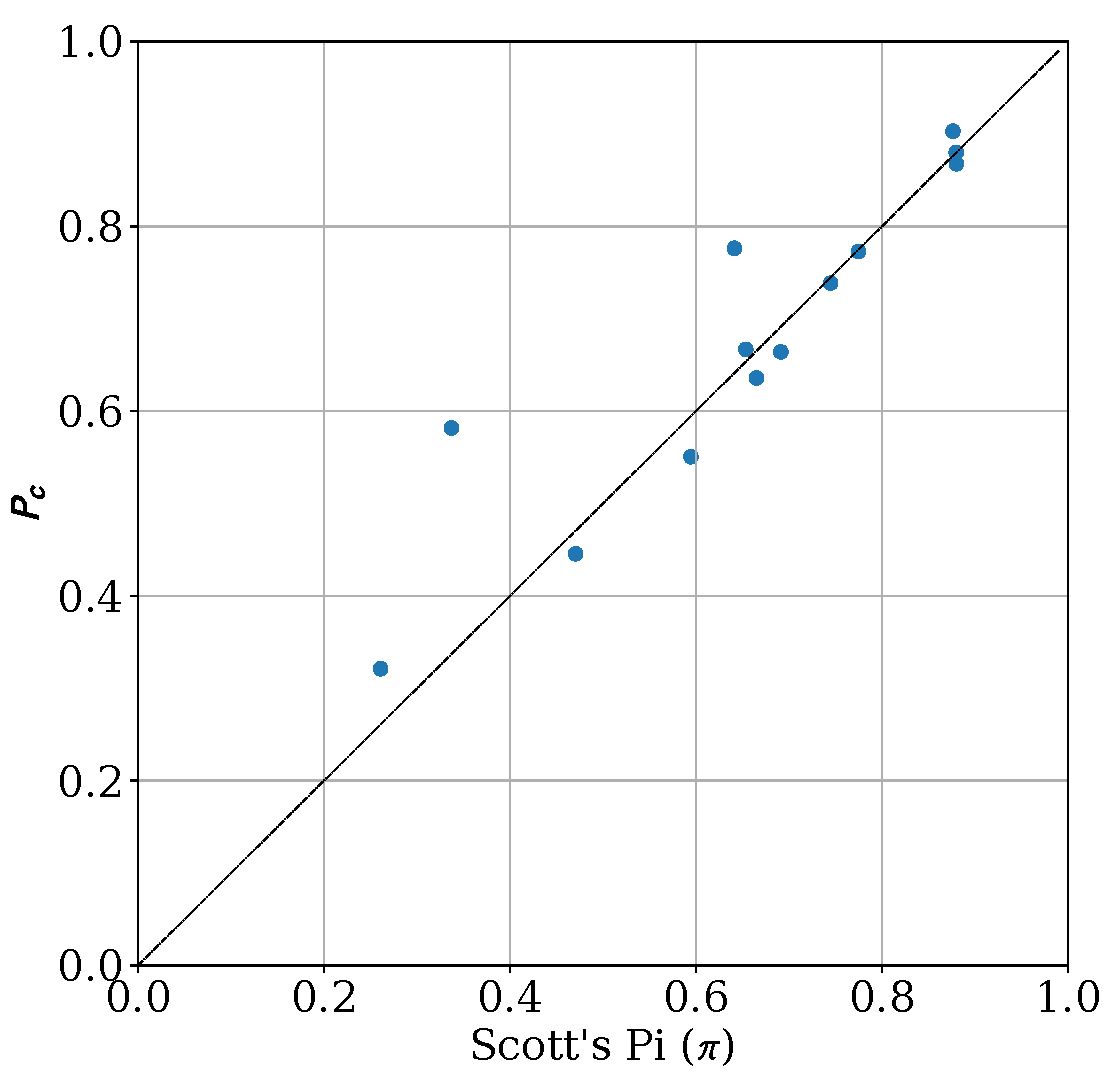
\includegraphics[width=\linewidth]{figures/corr9.pdf}
  \caption{}
  \label{fig:k-p-corr}
\end{subfigure}
\caption{a) Estimated values of $P_c$ and $P_+$ for different \judgemodels. b) Pearson's correlation coefficient between $\pi$ and $P_c$ for \judgemodels.}
\label{fig:leniency-bias-full}
\end{figure}

\begin{figure}[t]
    \centering
    \begin{subfigure}[b]{0.4\textwidth}
        \centering
        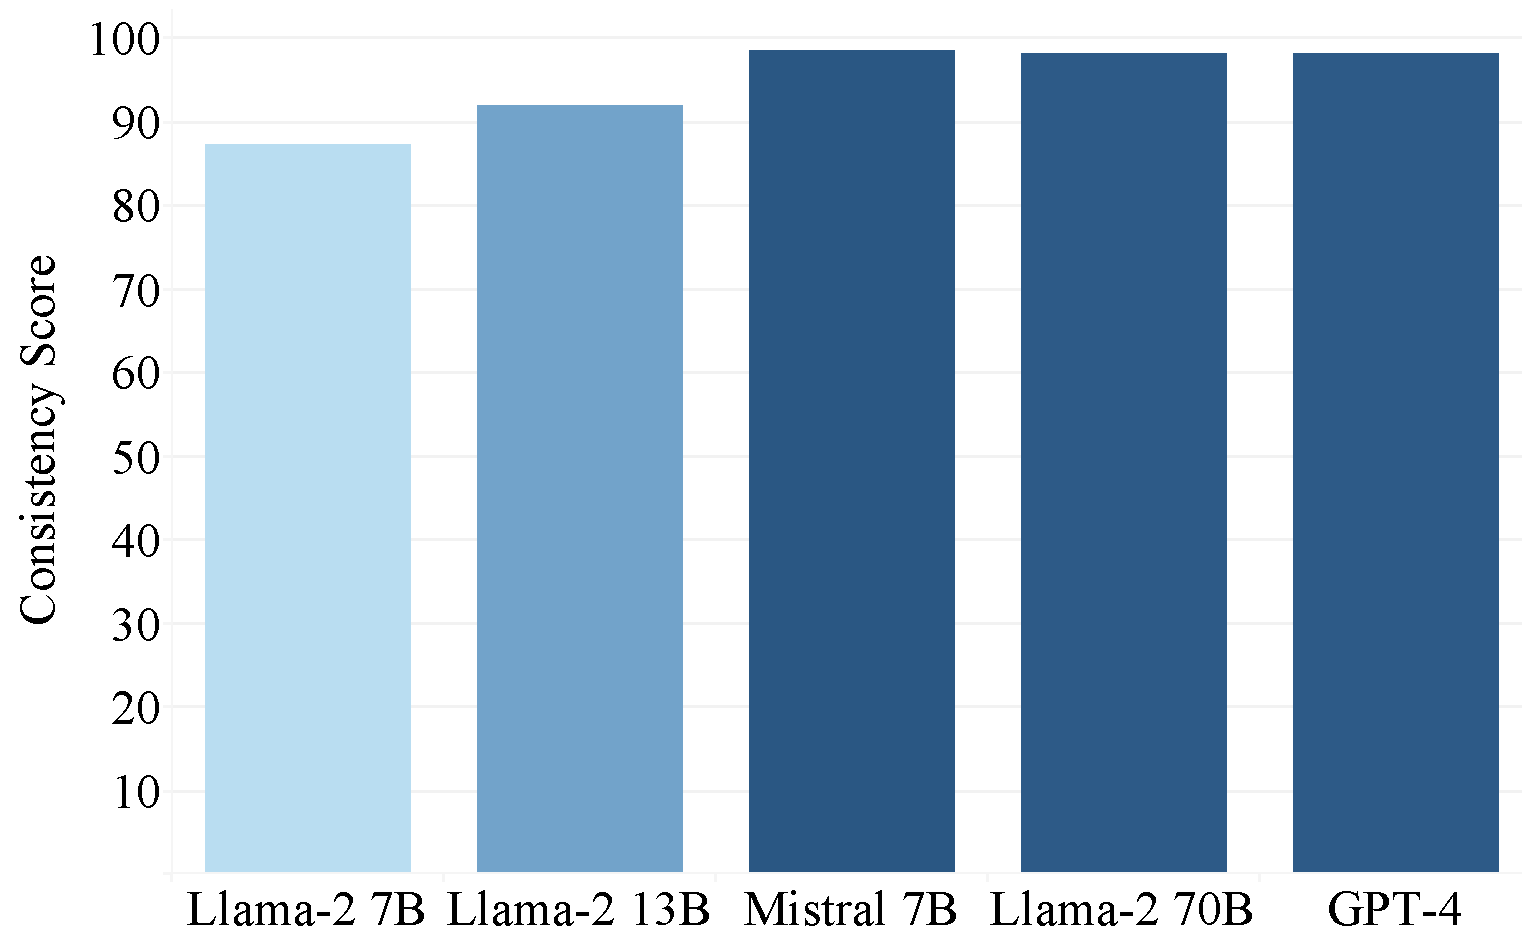
\includegraphics[width=\textwidth]{figures/Consistency.pdf}
        \label{fig:consistency}
    \end{subfigure}
    \caption{\textbf{Leniency bias and answer consistency.} Consistency score, defined as the percentage of questions for which the \judgemodel gives the same judgment for three different answer orders.}
\end{figure}

% \section{Evaluating base versus chat models} \label{sec:analysis:subsec:basevschat}

% \begin{table}[ht]
% \centering
% \vspace{0.5em} % Adjust the spacing here
% \begin{tabular}{ccccc}
% \multicolumn{1}{c}{\rule{0pt}{1em}} & \multicolumn{1}{c}{\rule{0pt}{1em}\judge{Human}} & \multicolumn{1}{c}{\rule{0pt}{1em}\judge{GPT}} & \multicolumn{1}{c}{\rule{0pt}{1em}\judge{Llama2-70B}} & \multicolumn{1}{c}{\rule{0pt}{1em}\judge{Llama2-7B}}\\ \hline
% \toprule\toprule
% Llama 7B & \rule{0pt}{1em}6.75 & \rule{0pt}{1em}9.5 & \rule{0pt}{1em}4.75 & \rule{0pt}{1em}1.75\\ 
% \midrule
% Mistral 7B & \rule{0pt}{1em}10.75 & \rule{0pt}{1em}11.5 & \rule{0pt}{1em}7.5  & \rule{0pt}{1em}6.25\\
% \midrule
% Llama 13B & \rule{0pt}{1em}16.5 & \rule{0pt}{1em}9 & \rule{0pt}{1em}3.75 & \rule{0pt}{1em}3.75\\
% \midrule
% Llama 70B & \rule{0pt}{1em}10 & \rule{0pt}{1em}10.25 & \rule{0pt}{1em}10  & \rule{0pt}{1em}7 \\
% \bottomrule
% \end{tabular}
% \vspace{1em} % Adjust the spacing between caption and table
% \caption{Difference in Evaluation Scores between different Base - Chat \evaluatormodel pairs for different \judgemodels}
% \label{tab:BasevsChat}
% \end{table} 
